% Training.tex: Training for hiragana and katakana
\ifthenelse{\equal{katakana}{\jtopic}}{%
\chapter{Katakana Training}\jchap{片仮名練習}\label{chap:KatakanaTraining}
\ithree{katakana!training}{片仮名練習}{Katakana!Training}
}{}
\ifthenelse{\equal{hiragana}{\jtopic}}{%
\chapter{Hiragana Training}\jchap{平仮名練習}\label{chap:HiraganaTraining}
\ithree{katakana!training}{平仮名練習}{Hiragana!Training}
}{}

\normalsize

Every person is learning in a different way. What works well for one does not
need to work well also for the other. Because of this an ultimate recipe to
learn \textbf{\jtopic} can not be given here. However the introduction to this
chapter would like to try to give some  hints gathered from learning and
teaching experience.

\begin{description}

\item[Not too less:] If one learns one character per day, it will take for
        \textbf{\jtopic} roughly \jkanacount{} days. If you restrict this to
        working days it will take approximately two month. If you restrict it
        to a 2h lesson per week it will take a year to learn \textbf{\jtopic}.
        It is obvious that one is likely to forget the first characters when
        learning the last. However, even with this method it is not impossible
        but not likely.

\item[Not too much:]  To learn \textbf{\jtopic} in one day is unlikely
        possible. At least parts will be forgotten the next day.

\end{description}

From the practice the best results have been seen when learners have tried to
learn \textbf{\jtopic} in one to three weeks. The suggestion is to learn one
line (five characters) per day in a cumulative way. Means, repeat every day the
already learned characters and that up to 10 days until all are learned. And
then repeat this exercise until they hardly can not be forgotten any more. So
for at least 14 consecutive days without break.

\begin{description}

\item[Develop your own style:] Learning one character at a time or a row (five
        characters at a time) or learn the whole table of \textbf{\jtopic} is
        possible. With some method it can take 3 weeks or with an other method
        1 week. That does not matter. What do matter is that oneself is
        comfortable with the method and that oneself extract fun out of it,
        even when forced to learn \textbf{\jtopic}. Decide by yourself how
        often you repeat. But decide. And write down your decision. Maybe even
        plan it in your daily plan. A good practice is to learn
        \textbf{\jtopic} 20 times a day for five minutes rather then one time
        for three hours a day or one time a week for 10 hours.

\item[Search for aid:] Aid can come in may manifestations. Of course it is
        useful to ask a Japanese to help. But there are many other ways for
        helping yourself.  One example are flashcards. Of course it is easy to
        print them in this book. However as said before: find your own way. And
        if you create flashcards by yourself you already learn the content up
        to a certain level.

\item[Use Squares:] Some European languages uses lines to teach letters. In
        Japanese you should use a square and draw the letter in the middle. If
        uncertain about the shape and orientation of the character use a square
        and look at the squares filled with \textbf{\jtopic} in this section to
        understand the alignment and orientation.

\end{description}

\newpage

Here are some examples for flashcards. But feel free to invent your own.

\begin{figure}[H]
        

\begin{center}
\begin{tabular}{cc}
\textbf{Front site rōmaji}&\textbf{Back site katakana}\\
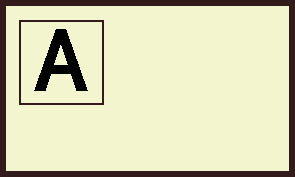
\includegraphics[scale=1.5]{../share/i/fcar.pdf}% Rōmaji
&
\ifthenelse{\equal{hiragana}{\jtopic}}{
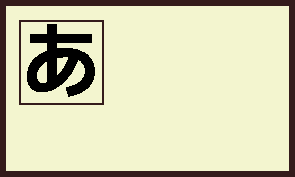
\includegraphics[scale=1.5]{../share/i/fcah.pdf}% Hiragana
}{}
\ifthenelse{\equal{katakana}{\jtopic}}{
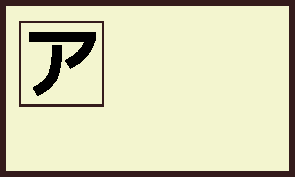
\includegraphics[scale=1.5]{../share/i/fcak.pdf}% Katakana
}{}
\\
\end{tabular}
\end{center}

        \caption{Flashcard type 1 (rōmaji - kana) }
        \label{fig:FlashCardTypeOne}
\end{figure}

\normalsize

Or to learn both:

\begin{figure}[H]
        \begin{center}
\begin{tabular}{cc}
\textbf{Front site rōmaji}&\textbf{Back site both}\\
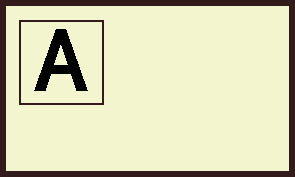
\includegraphics[scale=1.5]{../share/i/fcar.pdf}% Rōmaji
&
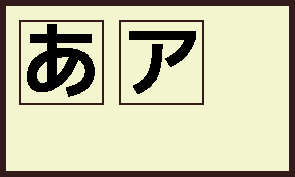
\includegraphics[scale=1.5]{../share/i/fcahk.pdf}% Hiragana/ Katakana
\\
\end{tabular}
\end{center}

        \caption{Flashcard type 2 (rōmaji - 2 kana)}
        \label{fig:FlashCardTypeTwo}
\end{figure}

\normalsize

To dive deep into Japanese of course skipping rōmaji is the preferred method:

\begin{figure}[H]
        \begin{center}
\begin{tabular}{cc}
\textbf{Front site Katakana}&\textbf{Back site Hiragana}\\
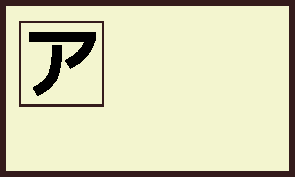
\includegraphics[scale=1.5]{../share/i/fcak.pdf}% Katakana
&
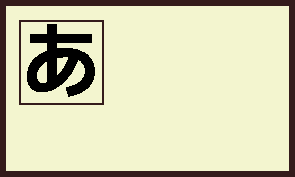
\includegraphics[scale=1.5]{../share/i/fcah.pdf}% Hiragana
\\
\end{tabular}
\end{center}

        \caption{Flashcard type 3 (katakana - hiragana)}
        \label{fig:FlashCardTypeThree}
\end{figure}

This training chapter can be used as an additional aid to learn
\textbf{\jtopic}. And also here it is important to develop ones own method.
However some hints on learning with this training chapter can be given.

\begin{description}

\item[Reading Loud:] While writing a \textbf{\jtopic} character in this book
        (and probably also later), read out loud the sound of the character.
        Always.

\item[Invent your own cribs:] One can (maybe should?) invent one crib per
        character by oneself. Especially if the characters is difficult to
        remember. It might be useful to write it down on the self created
        flashcard for that specific character.

\item[Regular Repetition:] It is of course possible to fill out all fields for
        one character in a very short time. The learning effect should be
        minimal though. Better is to fill out one row and then the second row
        an hour later, the third row the next day and so own. Oneself has to
        decide the rhythm of the repetition.

\item[Transcription:]  Search for a  \textbf{\jtopic} text and read it. Write
        for every \jtopic word the Roman letters. If this is possible without
        looking up the \jtopic, then the transcription should be reversed. Find
        some Japanese text written in Rōmaji and transcribe them to \jtopic on
        a different piece of paper.

\end{description}

\newpage

                                             % Katakana Hiragana
%----------------------------------------------------------------------------
\section{Katakana /a/ Row}\jsec{ 片仮名ア行}\label{sec:KatakanaARow}

\Krow{arow}{a}{i}{u}{e}{o}

\label{letter:a}\KLETTER{a} The 片仮名 {「ア」} derives from the
\hyperref[sec:PhoneticCharacter]{Phonetic Characters}
(\hyperref[sec:Radical]{radical}).  A smaller version {「ァ」} is used in
combinations with other letters as {「ファ」} and is pronounced as /fa/ in
\hyperref[sec:Hepburn]{Hepburn} transcription.

\label{letter:i}\KLETTER{i} The 片仮名 {「イ」} derives from the
\hyperref[sec:PhoneticCharacter]{Phonetic Characters} {「伊」} left element
(\hyperref[sec:Radical]{radical}).  A smaller version {「ィ」} is used in
combinations with other letters and represents a
\hyperref[sec:Diphthong]{diphthong}. 

\label{letter:u}\KLETTER{u} The 片仮名 {「ウ」} derives from the
\hyperref[sec:PhoneticCharacter]{Phonetic Character} {「宇」}. A smaller version
{「ゥ」} is used in combinations with other letters and represents a
\hyperref[sec:Diphthong]{diphthong} and is written as "w". Even though the
combination {「トゥ」} /tu/ exist, it is relatively new and many words do not
use it. In this cases {「ツ 」} /tsu/ is used. {「ウ」} can take
\hyperref[sec:Dakuten]{Dakuten} to form {「ヴ」} /vu/, which is relatively new
and can replace {「ブ」} /bu/. 

\Note{Note}{%

Be aware that the characters \hyperref[letter:fu]{「フ」},
\hyperref[letter:wa]{「ワ」}  and \hyperref[letter:u]{「ウ」} look very
similar.  Make sure that you spend extra training on distinguish them. 

}%


\newpage 

\label{letter:e}\KLETTER{e} The 片仮名 {「エ」} derives from the
\hyperref[sec:PhoneticCharacter]{Phonetic Characters} {「江」} right element
(\hyperref[sec:Radical]{radical}). A smaller version {「ェ」} is used in
combinations with other letters and express \hyperref[sec:Mora]{morae} of
foreign origin. For example {「ヴェ」} as pronounced /ve/.

\label{letter:o}\KLETTER{o} The 片仮名 {「オ」} derives from the
\hyperref[sec:PhoneticCharacter]{Phonetic Character} {「於」}. A smaller version
{「ォ」} is used in combinations with other letters and express
\hyperref[sec:Mora]{morae} of foreign origin. For example {「フォ 」} as
pronounced /fo/.

\newpage

% ---------------------------------------------------------------------------
\subsection{/a/}\jsubsec{「ア」} \label{sec:KatakanaA}

\KatakanaHeader{a}{ The Katakana {「ア」} is written with two strokes. The
first stroke starts horizontal. The second stroke is a curve with can be
attached to the first stroke in hand writing, but not at the horizontal part -
at the end of the first line.} \KatakanaTraining{a}

% ---------------------------------------------------------------------------
\subsection{/i/}\jsubsec{「イ」} \label{sec:KatakanaI}

\KatakanaHeader{i}{ The Katakana {「イ」} is written with one stroke. The first
stroke is a curve from upper right to lower left. The second stroke is a
vertical line attached to the first at the top.} \KatakanaTraining{i}

% ---------------------------------------------------------------------------
\subsection{/u/}\jsubsec{「ウ」} \label{sec:KatakanaU}

\KatakanaHeader{u}{The Katakana {「ウ」} is written with three strokes. The
first stroke a small vertical line. The second a small vertical line again and
the third line a horizontal line connection the two others.}
\KatakanaTraining{u}

% ---------------------------------------------------------------------------
\subsection{/e/}\jsubsec{「エ」} \label{sec:KatakanaE}

\KatakanaHeader{e}{The Katakana {「エ」} is written with three strokes. It is
very geometrically consisting only out of horizontal and vertical lines
connected together.} \KatakanaTraining{e}

% ---------------------------------------------------------------------------
\subsection{/o/}\jsubsec{「オ」} \label{sec:KatakanaO}

\KatakanaHeader{o}{The Katakana {「オ」} is written with three strokes. The
first line is horizontal and together with the second stroke it constructs a
perfect crossing. The third stroke beginning lies at the center of the
crossing.} \KatakanaTraining{o}

% ---------------------------------------------------------------------------
\subsection{/a/ Row Training}\jsubsec{片仮名ア行練習}
\Padding
\begin{longtable}[c]{p{2cm}p{2cm}p{3cm}p{6cm}p{2cm}}
\textit{Katakana}&\textit{Rōmaji}&\textit{Original}&\textit{Remark}&Origin\\\hline
ウエア&wuea&ware&          &English\\
エア  &ea  &air &          &English\\
エイ  &ei  &A   &the letter&English\\
\end{longtable}

\KanaSimpleTraining{Katakana to Rōmaji}{
\Transcribe{1.}{ウエア}{}{wear, ware}
\Transcribe{2.}{エア}{}{air}
\Transcribe{3.}{エイ}{}{A (the letter)}
\Transcribe{4.}{アイ}{}{I (the letter)}
\Transcribe{5.}{オウ}{}{O (the letter)}
%\Transcribe{6.}{イア}{}{ear}
}

\KanaSimpleTraining{Rōmaji to Katakana}{
\Transcribe{1.}{ea}{}{air}
\Transcribe{2.}{ai}{}{I (the letter)}
\Transcribe{3.}{ou}{}{O (the letter)}
\Transcribe{4.}{ei}{}{A (the letter)}
\Transcribe{5.}{uea}{}{wear, ware}
%\Transcribe{6.}{ia}{}{ear}
}

\newpage
\Padding
\begin{longtable}[c]{p{2cm}p{2cm}p{3cm}p{6cm}p{2cm}}
\textit{Katakana}&\textit{Rōmaji}&\textit{Original}&\textit{Remark}&Origin\\\hline
アイ  &ai  &I   &the letter&English\\
オウ  &ou  &O   &the letter&English\\
イア  &ia  &ear &          &English\\
\end{longtable}

\KanaSimpleTraining{English to Rōmaji}{
\Transcribe{1.}{ear}{}{}
\Transcribe{2.}{I (the letter)}{}{}
\Transcribe{3.}{air}{}{}
\Transcribe{4.}{O (the letter)}{}{}
\Transcribe{5.}{wear, ware}{}{}
%\Transcribe{6.}{A (the letter)}{}{}
}

\KanaSimpleTraining{English to Katakana}{
\Transcribe{1.}{I (the letter)}{}{}
\Transcribe{2.}{O (the letter)}{}{}
\Transcribe{3.}{air}{}{}
\Transcribe{4.}{ear}{}{}
\Transcribe{5.}{wear, ware}{}{}
%\Transcribe{6.}{A (the letter)}{}{}
}
\newpage
   % OK       OK
% ---------------------------------------------------------------------------
\section{Katakana \jtl{ka} Row}\jsec{片仮名カ行}\label{sec:KatakanaKaRow}

\Krow{karow}{ka}{ki}{ku}{ke}{ko}

\label{letter:ka}\KLETTER{ka} The  \textbf{katakana} \jquotesingleja{カ} is
pronounced \jtl{ka} and  derives from the
\hyperref[sec:PhoneticCharacter]{phonetic character}s \jquotesingleja{加} left
\hyperref[sec:Radical]{radical}.  A \hyperref[sec:Dakuten]{dakuten} version
exists and pronounced as \jtl{ga}.

%\hyperref[sec:Handakuten]{handakuten} does not exist in daily Japanese.
% \jquotesingleja{一ヵ所} {【いちかしょ】} (one place)
% \jquotesingleja{一ヶ所} {【いちかしょ】} (one place).
% 十ヵ条(十ヶ条)

\Note{Note}{

A smaller version \jquotesingleja{ヵ} is rare but used in combinations with
number particles.  For example in \jquotesingleja{一ヵ月} {【いっかげつ】} (one
month) and others.  This cases can also be written \jquotesingleja{一ヶ月}
{【いっかげつ】} (one month). Please see also \nameref{sec:KatakanaKe}. \Link
\href{https://ja.wikipedia.org/wiki/\%E3\%83\%B5}{ヵ}

}

\label{letter:ki}\KLETTER{ki} The \textbf{katakana} \jquotesingleja{キ} derives
from the \hyperref[sec:PhoneticCharacter]{phonetic character}s middle part of
either \jquotesingleja{機} or \jquotesingleja{幾}.  It is pronounced as
\jtl{ki}.  A \hyperref[sec:Dakuten]{dakuten} version exists and pronounced as
\jtl{gi}.


\label{letter:ku}\KLETTER{ku} The \textbf{katakana} \jquotesingleja{ク} derives
from the \hyperref[sec:PhoneticCharacter]{phonetic character}s left upper part
of \jquotesingleja{久}.  It is pronounced as \jtl{ku}.  A
\hyperref[sec:Dakuten]{dakuten} version exists and pronounced as \jtl{gu}.  A
smaller version exists, but is used for the Ainu Language.

\label{letter:ke}\KLETTER{ke} The \textbf{katakana} \jquotesingleja{ケ} derives
from the \hyperref[sec:PhoneticCharacter]{phonetic character}s upper and left
part of \jquotesingleja{介}.  It is pronounced as \jtl{ke}.  A
\hyperref[sec:Dakuten]{dakuten} version exists and pronounced as \jtl{ge}.  The
smaller version \jquotesingleja{ヶ} is explained in the following note.

\newpage

\Note{Note}{

A smaller version \jquotesingleja{ヶ} is rare but used in combinations with
number particles.  For example in \jquotesingleja{一ヶ月} {【いっかげつ】} (one
month) and others.  This cases can also be written \jquotesingleja{一ヵ月}
{【いっかげつ】} (one month). There are cases where only \jquotesingleja{ヶ}
can be written {七ヶ宿} {【シチカシュク】} (Place at the south west border of
the prefecture Miyagi).  In other rare cases this character can be pronounced
different \jquotesingleja{関ヶ原} {【せきがはら】} (Place at the south border
of the Gifu prefecture, known by the battle at 1600.). Please see also
\nameref{sec:KatakanaKa}. \Link
\href{https://ja.wikipedia.org/wiki/\%E3\%83\%B5}{ヵ}

}

\label{letter:ko}\KLETTER{ko} The \textbf{katakana} \jquotesingleja{コ} derives
from the \hyperref[sec:PhoneticCharacter]{phonetic character}s upper part of
\jquotesingleja{己}.  It is pronounced as \jtl{ko}.  A
\hyperref[sec:Dakuten]{dakuten} version exists and pronounced as \jtl{go}.



\newpage

% ---------------------------------------------------------------------------
\subsection{\jtl{ka}}\jsubsec{\jquotesingleja{カ}} \label{sec:KatakanaKa}

\KatakanaHeader{ka}{ \jtl{ka} is written with 2 strokes. Basically the same way
as the Hiragana \jquotesingleja{か} it looks like a squarish version, but
without the last stroke. The hook at the second stroke is less significant or
important.  } \KatakanaTraining{ka}

% ---------------------------------------------------------------------------
\subsection{\jtl{ki}}\jsubsec{\jquotesingleja{キ}} \label{sec:KatakanaKi}

\KatakanaHeader{ki}{ The shape alignment of the \jquotesingleja{キ} character
is not straight towards its environment. However the junctions are more or less
90 degrees.  } \KatakanaTraining{ki}

% ---------------------------------------------------------------------------
\subsection{\jtl{ku}}\jsubsec{\jquotesingleja{ク}} \label{sec:KatakanaKu}
% ---------------------------------------------------------------------------

\KatakanaHeader{ku}{ The first stroke is similar the stroke of
\jquotesingleja{ケ} is a curve. While the second stroke start aligned and
straight. } \KatakanaTraining{ku}

% ---------------------------------------------------------------------------
\subsection{\jtl{ke}}\jsubsec{\jquotesingleja{ケ}} \label{sec:KatakanaKe}

\KatakanaHeader{ke}{ The \jquotesingleja{ケ} is written with 3 strokes and the
first stroke is similar to the \jquotesingleja{ク}. The second stroke is
aligned and straight.  While the last stroke is a curve.  }
\KatakanaTraining{ke}

% ---------------------------------------------------------------------------
\subsection{\jtl{ko}}\jsubsec{\jquotesingleja{コ}} \label{sec:KatakanaKo}

\KatakanaHeader{ko}{ This character is almost a geometric figure composed out
of two strokes. However unless in European languages this are only 2 strokes
and not 3. The first stroke is the longest one and done similar with all
{漢字}. } \KatakanaTraining{ko}

% ---------------------------------------------------------------------------
\subsection{\jtl{ka} Row Training}\jsubsec{片仮名カ行練習}

\Padding
\begin{longtable}[c]{p{2cm}p{1.5cm}p{1.5cm}p{3cm}p{7cm}}
\textit{Katakana}&\textit{Rōmaji}&\textit{Original}&\textit{Remark}&Origin\\\hline
カキ  &kaki &kaki &柿 persimon&Japanese\\
ケア  &kea  &care &          &English\\
ケイ  &kei  &K    &the letter&English\\
\end{longtable}

\KanaSimpleTraining{Katakana to Rōmaji}{
\Transcribe{1.}{カキ}{}{persimmon}
\Transcribe{2.}{ココア}{}{cocoa}
\Transcribe{3.}{ケア}{}{care}
\Transcribe{4.}{コア}{}{core}
\Transcribe{5.}{ケーキ}{}{cake}
%\Transcribe{6.}{ケイ}{}{K (the letter)}
}

\KanaSimpleTraining{Rōmaji to Katakana}{
\Transcribe{1.}{kokoa}{}{cocoa}
\Transcribe{2.}{k$\overline{\mbox{e}}$ki}{}{cake}
\Transcribe{3.}{kea}{}{care}
\Transcribe{4.}{koa}{}{core}
\Transcribe{5.}{kaki}{}{persimmon}
%\Transcribe{6.}{kei}{}{K (the letter)}
}

\newpage

\Padding
%\begin{longtable}[c]{p{2cm}p{2cm}p{3cm}p{6cm}p{2cm}}
\begin{longtable}[c]{p{2cm}p{2.0cm}p{3.5cm}p{4cm}p{2.5cm}}
\textit{Katakana}&\textit{Rōmaji}&\textit{Original}&\textit{Remark}&Origin\\\hline
コア  &koa  &core &          &English\\
ココア&kokoa&cocoa& hot chocolate &English, from metathesis of Spanish cacao, from Nahuatl cacahuatl\\
ケーキ&kēki &cake &          &English\\
\end{longtable}


\KanaSimpleTraining{English to Rōmaji}{
\Transcribe{1.}{persimon}{}{}
\Transcribe{2.}{cocoa}{}{}
\Transcribe{3.}{care}{}{}
\Transcribe{4.}{core}{}{}
\Transcribe{5.}{K (the letter)}{}{}
%\Transcribe{6.}{cake}{}{}
}

\KanaSimpleTraining{English to Katakana}{
\Transcribe{1.}{cocoa}{}{}
\Transcribe{2.}{cake}{}{}
\Transcribe{3.}{care}{}{}
\Transcribe{4.}{persimon}{}{}
\Transcribe{5.}{K (the letter)}{}{}
%\Transcribe{6.}{core}{}{}
}

\newpage
  % OK
%----------------------------------------------------------------------------
\section{Katakana /sa/ Row}\jsec{片仮名サ行}\label{sec:KatakanaSaRow}

\Krow{sarow}{sa}{shi}{su}{se}{so}

\label{letter:sa}\KLETTER{sa} The  片仮名 {「サ」} is pronounced  /sa/ and
derives from the \hyperref[sec:PhoneticCharacter]{Phonetic Character}s {「散」}
upper left corner \hyperref[sec:Radical]{radical}.  A
\hyperref[sec:Dakuten]{濁点} version exists and pronounced as /za/.

\label{letter:shi}\KLETTER{shi} The 片仮名 {「シ」} derives from the
\hyperref[sec:PhoneticCharacter]{Phonetic Character}  {「之 」}.  It is
pronounced as /shi/.  A \hyperref[sec:Dakuten]{濁点} version exists and
pronounced as /ji/.

\Note{Note}{Please see section \nameref{subsec:ShiTsuAmbiguity} for the
explanation how to write and distinguish /shi/ and /tsu/.  }

\label{letter:su}\KLETTER{su} The 片仮名 {「ス」} derives from the
\hyperref[sec:PhoneticCharacter]{Phonetic Character}s right lower part of
{「須」}.  It is pronounced as /su/.  A \hyperref[sec:Dakuten]{濁点} version
exists and pronounced as /zu/.

\label{letter:se}\KLETTER{se} The 片仮名 {「セ」} derives from the
\hyperref[sec:PhoneticCharacter]{Phonetic Character}s middle left part of
{「世」}.  It is pronounced as /se/.  A \hyperref[sec:Dakuten]{濁点} version
exists and pronounced as /ze/.

\newpage

\label{letter:so}\KLETTER{so} The 片仮名 {「ソ」} derives from the
\hyperref[sec:PhoneticCharacter]{Phonetic Character}s upper right part of
{「曽」}.  It is pronounced as /so/.  A \hyperref[sec:Dakuten]{濁点} version
exists and pronounced as /zo/.

% SoRiNAmbiguity
\subsection{|so|, |ri| and |n| Ambiguity} \label{subsec:SoRiNAmbiguity}

The Katakana characters {「ソ」}, {「リ」} and {「ン」} can be difficult to
distinguish. All three are made out of only 2 strokes. And especially |so| and
|n| can be hard to tell. In a sentence of course the context can help a lot.
But what are the rules for this characters to write properly and distinguish?

\bigskip

\begin{center}
\begin{tabular}{|c|c|c|}\hline
\KLETTER{so}&\KLETTER{n}&\KLETTER{ri}\\\hline
\end{tabular}
\end{center}

\CharacterExplanation{soexplanation}{ To write the letter |so| it is important
to align both lines \textbf{horizontally} (red line) and to \textbf{non-align}
the ends (blue line) vertically. In this way it is possible to distinguish |so|
from |n|, but not from |ri|. To also distinguish it from |ri| you have to write
the first stroke not horizontally nor vertically (green line).  }

\CharacterExplanation{nexplanation}{ To write the letter |n| it is important to
a align both lines \textbf{vertically} (red line) and to \textbf{non-align} the
ends (blue line). In this way it is possible to distinguish |n| from |so|. If
both lines are aligned there should not be a problem to distinguish it from
|ri|. Usually the angle of the green line is different, but only a small
indicator. }

\CharacterExplanation{riexplanation}{ To write the letter |ri| it is important
to \textbf{align} both of the line beginnings \textbf{horizontally} (red line)
and to make sure that both lines are \textbf{parallel} (green lines). There
should be \textbf{no alignment} on the left side (blue line)
\textbf{vertically}. The difference between |so| and |ri| is that |ri| need to
start with two \textbf{parallel} lines wile |so| should not. Please compare the
left green line for an explanation.  }



\newpage
% ---------------------------------------------------------------------------
\subsection{/sa/}\jsubsec{「サ」}\label{sec:KatakanaSa}

\KatakanaHeader{sa}{ Katakana {「サ」} is written with three strokes. All
crossings of strokes are in a 90 degree angle.  The starts of all strokes are
aligned eitehr horizontally or vertically. The last stroke has a curve.}
\KatakanaTraining{sa}

% ---------------------------------------------------------------------------
\subsection{/shi/}\jsubsec{「シ」}\label{sec:KatakanaShi}

\KatakanaHeader{shi}{ The Katakana {「シ」} is written with three strokes. All
three strokes are aligned vertically in the beginning. Please see section
\nameref{subsec:ShiTsuAmbiguity}.} \KatakanaTraining{shi}

% ---------------------------------------------------------------------------
\subsection{/su/}\jsubsec{「ス」}\label{sec:KatakanaSu}

\KatakanaHeader{su}{The Katakana {「ス」} is written with two strokes. The
first stroke startes horizontally aligned. The second stroke touches the first
stroke at the beginning.} \KatakanaTraining{su}

% ---------------------------------------------------------------------------
\subsection{/se/}\jsubsec{「セ」}\label{sec:KatakanaSe}

\KatakanaHeader{se}{ The Katakana {「セ」} is written with two strokes. The
crossing has \textbf{no} 90 degree angle. The curve of the second stroke as
almost a 90 deegre angle. } \KatakanaTraining{se}

% ---------------------------------------------------------------------------
\subsection{/so/}\jsubsec{「ソ」}\label{sec:KatakanaSo}

\KatakanaHeader{so}{ The Katakana {「ソ」} is written with two strokes. The
first stroke is not aligned verticall but it is aligned horizontally withe the
second stroke. Please see section \nameref{subsec:SoRiNAmbiguity}.}
\KatakanaTraining{so}

% ---------------------------------------------------------------------------
\subsection{/sa/ Row Training}\jsubsec{片仮名サ行練習}\label{sec:SaRowTraining}
% 3 78 エキス
%3 357 スカイ
%3 360 スキー
%3 3 アイス
%3 111 ガーゼ
%3 146 イエス
\Padding
\begin{longtable}[c]{p{2cm}p{2cm}p{3cm}p{6cm}p{2cm}}
\textit{Katakana}&\textit{Rōmaji}&\textit{Original}&\textit{Remark}&\textit{Origin}\\\hline
エキス&ekisu&ex(tract)&extract&Dutch\\
スカイ&sukai&sky&&English\\
スキー&sukī&ski&noun for skiing&English\\
\end{longtable}
\KanaSimpleTraining{Katakana to Rōmaji}{
\Transcribe{1.}{エキス}{}{extract}      % ekisu
\Transcribe{2.}{スカイ}{}{sky}          % sukai
\Transcribe{3.}{スキー}{}{ski}          % sukī
\Transcribe{4.}{アイス}{}{ice}          % aisu
\Transcribe{5.}{ガーゼ}{}{gauze}        % gāze
%\Transcribe{6.}{イエス}{}{Jesus}        % iesu
}

\KanaSimpleTraining{Rōmaji to Katakana}{
\Transcribe{1.}{sukai}{}{sky}         % sukai
\Transcribe{2.}{ekisu}{}{extract}     % ekisu
\Transcribe{3.}{aisu}{}{ice}          % aisu
\Transcribe{4.}{suki}{}{ski}          % sukī
\Transcribe{5.}{iesu}{}{Jesus}        % iesu
%\Transcribe{6.}{gāze}{}{gauze}        % gāze
}

\newpage

\Padding
\begin{longtable}[c]{p{2cm}p{2cm}p{3cm}p{6cm}p{2cm}}
\textit{Katakana}&\textit{Rōmaji}&\textit{Original}&\textit{Remark}&Origin\\\hline
アイス&aisu&ice&water ice, ice cream&English\\
ガーゼ&gāze&Gaze&gauze&German\\
イエス&iesu&Jesus&Jesus&Portuguese\\
\end{longtable}
\KanaSimpleTraining{English to Rōmaji}{
\Transcribe{1.}{extract}{}{}       % ekisu
\Transcribe{2.}{sky}{}{}           % sukai
\Transcribe{3.}{Jesus}{}{}         % iesu
\Transcribe{4.}{gauze}{}{}         % gāze
\Transcribe{5.}{ice}{}{}           % aisu
%\Transcribe{6.}{ski}{}{}           % sukī
}

\KanaSimpleTraining{English to Katakana}{
\Transcribe{1.}{sky}{}{}           % sukai
\Transcribe{2.}{gauze}{}{}         % gāze
\Transcribe{3.}{ice}{}{}           % aisu
\Transcribe{4.}{Jesus}{}{}         % iesu
\Transcribe{5.}{extract}{}{}       % ekisu
%\Transcribe{6.}{ski}{}{}           % sukī
}

\newpage
  % OK
% ---------------------------------------------------------------------------
\section{Katakana \jtl{ta} Row}\jsec{片仮名タ行}\label{sec:KatakanaTaRow}

\Krow{tarow}{ta}{chi}{tsu}{te}{to}

\label{letter:ta}\KLETTER{ta} The  \textbf{katakana} \jquotesingleja{タ} is
pronounced \jtl{ta} and derives from the
\hyperref[sec:PhoneticCharacter]{phonetic character}s \jquotesingleja{多 }
upper or lover \hyperref[sec:Radical]{radical}.  A
\hyperref[sec:Dakuten]{dakuten} version exists and pronounced as \jtl{da}.

\label{letter:chi}\KLETTER{chi} The \textbf{katakana} \jquotesingleja{チ}
derives from the \hyperref[sec:PhoneticCharacter]{phonetic character} 
\jquotesingleja{千}.  It is pronounced as \jtl{chi}.  A
\hyperref[sec:Dakuten]{dakuten} version exists and pronounced as \jtl{ji}.

\label{letter:tsu}\KLETTER{tsu} The \textbf{katakana} \jquotesingleja{ツ}
derives from the \hyperref[sec:PhoneticCharacter]{phonetic character}s
\jquotesingleja{州} or \jquotesingleja{川} .  It is pronounced as \jtl{tsu}.  A
\hyperref[sec:Dakuten]{dakuten} version exists and pronounced as \jtl{zu}.

\label{letter:te}\KLETTER{te} The \textbf{katakana} \jquotesingleja{テ} derives
from the \hyperref[sec:PhoneticCharacter]{phonetic character}s lower left part
of \jquotesingleja{天 }.  It is pronounced as \jtl{te}.  A
\hyperref[sec:Dakuten]{dakuten} version exists and pronounced as \jtl{de}.

\newpage

\label{letter:to}\KLETTER{to} The \textbf{katakana} \jquotesingleja{ト} derives
from the \hyperref[sec:PhoneticCharacter]{phonetic character}s right part of
\jquotesingleja{止}.  It is pronounced as \jtl{to}.  A
\hyperref[sec:Dakuten]{dakuten} version exists and pronounced as \jtl{do}.

% ShiTsuAmbiguity
\subsection{|shi| and |tsu| Ambiguity} \label{subsec:ShiTsuAmbiguity}

% シ
% ツ

The Katakana characters {「シ」} and {「ツ」} are difficult to distinguish.
Both are made out of 3 strokes and even the length are equal. In a sentence of
course the context can help a lot. But what are the rules for this characters
to write properly and distinguish?

\bigskip

\begin{center}
\begin{tabular}{|c|c|}\hline
\KLETTER{shi}&\KLETTER{tsu}\\\hline
\end{tabular}
\end{center}

\CharacterExplanation{shiexplanation}{ To write the letter |shi| it is
important to align three lines \textbf{vertically} (red line) and to
\textbf{non-align} the ends (blue line). In this way it is possible to
distinguish |shi| from |tsu|. Of course also the angle of the frist two lines
are different, but in hadwriting this is difficult to match. As a rule of thumb
make the third line double as long as the first two but short enough to not
align it at the end. }

\CharacterExplanation{tsuexplanation}{ To write the letter |tsu| it is
important to align all tree lines \textbf{horizontally} (red line) and to
\textbf{non-align} the ends (blue line). In this way it is possible to
distinguish |tsu| from |shi|. Of course also the angle of the first two lines
are different, but in handwriting this is difficult to match. As a rule of
thumb make the third line double as long as the first two but short enough to
not align it at the end. }



\newpage

% ---------------------------------------------------------------------------
\subsection{\jtl{ta}}\jsubsec{\jquotesingleja{タ}}\label{sec:KatakanaTa}

\KatakanaHeader{ta}{ Katakana \jtl{ta} is written with three strokes. The first
stroke is a small curve. The secosnd stroke starts horizontally attached to the
first stroke. The third stroke ends at the second stroke.}
\KatakanaTraining{ta}

% ---------------------------------------------------------------------------
\subsection{\jtl{chi}}\jsubsec{\jquotesingleja{チ}}\label{sec:KatakanaChi}

\KatakanaHeader{chi}{ Katakana \jtl{chi} is written with three strokes. The
first stroke is a light curve. The second ihorizontally straight line. The
third line is a curve that joints the first and the second.}
\KatakanaTraining{chi}

% ---------------------------------------------------------------------------
\subsection{\jtl{tsu}}\jsubsec{\jquotesingleja{ツ}}\label{sec:KatakanaTsu}

\KatakanaHeader{tsu}{Katakana \jtl{tsu} is written with three strokes. The
first and second stroke are short. And the beginning of all three strokes is
aligned horizontally. The third stroke is the longest, but the end is not
alignd wit the beginning of the first stroke. } \KatakanaTraining{tsu}

% ---------------------------------------------------------------------------
\subsection{\jtl{te}}\jsubsec{\jquotesingleja{テ}}\label{sec:KatakanaTe}

\KatakanaHeader{te}{ Katakana \jtl{te} is written with three strokes. The first
stroke is the shortest and horizontally. The second stroke is not aligned
vertically in the beginning, but also perfectly horizontally. The third stroke
is a small curve attached to the middle of the second stroke. }
\KatakanaTraining{te}

% ---------------------------------------------------------------------------
\subsection{\jtl{to}}\jsubsec{\jquotesingleja{ト}}\label{sec:KatakanaTo}

\KatakanaHeader{to}{ Katakana \jtl{to} is written with 2 strokes. The first
stroke is a vertical line. Attached to this line there is short straight line
to the right. In some hand writings this line is a small curve to the right.}
\KatakanaTraining{to}

% ---------------------------------------------------------------------------
\subsection{\jtl{ta} Row Training}\jsubsec{片仮名タ行練習}
\Padding
\begin{longtable}[c]{p{2cm}p{2cm}p{3cm}p{6cm}p{2cm}}
\textit{Katakana}&\textit{Rōmaji}&\textit{Original}&\textit{Remark}&\textit{Origin}\\\hline
エステ        &esutei    &esthé(tique)&beauty salon, esthetic clinic    &French\\
サイト        &saito     &site        &&English\\
タスク        &tasuku    &task        &&English\\
\end{longtable}

\KanaSimpleTraining{Katakana to Rōmaji}{
\Transcribe{1.}{エステ}{}{esthé(tique)}
\Transcribe{2.}{サイト}{}{site}
\Transcribe{3.}{タスク}{}{task}
\Transcribe{4.}{テスト}{}{test}
\Transcribe{5.}{スーツアクター}{}{suit actor}
%\Transcribe{6.}{テキスト}{}{text}
}

\KanaSimpleTraining{Rōmaji to Katakana}{
\Transcribe{1.}{saito}{}{site}
\Transcribe{2.}{tasuku}{}{task}
\Transcribe{3.}{esute}{}{esthé(tique)}
\Transcribe{4.}{sūtsuakutā}{}{suit actor}
\Transcribe{5.}{tesuto}{}{test}
%\Transcribe{6.}{テキスト}{}{text}
}

\newpage
\Padding
\begin{longtable}[c]{p{2.6cm}p{2cm}p{1.8cm}p{6.6cm}p{1.8cm}}
\textit{Katakana}&\textit{Rōmaji}&\textit{Original}&\textit{Remark}&\textit{Origin}\\\hline
テスト        &tesuto    &test        &                                 &English\\
スーツアクター&sūtsuakutā&suit actor  &wearing cartoon-character costume&English\\
テキスト      &tekisuto  &text        &                                 &English\\
\end{longtable}

\KanaSimpleTraining{English to Rōmaji}{
\Transcribe{1.}{task}{}{}
\Transcribe{2.}{esthé(tique)}{}{}
\Transcribe{3.}{text}{}{}
\Transcribe{4.}{test}{}{}
\Transcribe{5.}{suit actor}{}{}
%\Transcribe{6.}{site}{}{}
}

\KanaSimpleTraining{English to Katakana}{
\Transcribe{2.}{esthé(tique)}{}{}
\Transcribe{4.}{test}{}{}
\Transcribe{5.}{suit actor}{}{}
\Transcribe{3.}{text}{}{}
\Transcribe{6.}{site}{}{}
%\Transcribe{1.}{task}{}{}
}

\newpage
  % OK
% ---------------------------------------------------------------------------
\section{Katakana \jtl{na} Row}\jsec{片仮名ナ行}\label{sec:KatakanaNaRow}

\Krow{narow}{na}{ni}{nu}{ne}{no}

\label{letter:na}\KLETTER{na} The  \textbf{katakana} \jquotesingleja{ナ} is
pronounced \jtl{na} and  derives from the
\hyperref[sec:PhoneticCharacter]{phonetic character}s \jquotesingleja{奈} upper
left corner part.  A \hyperref[sec:Dakuten]{dakuten} version  or
\hyperref[sec:Handakuten]{handakuten} do not exist.

\label{letter:ni}\KLETTER{ni} The  \textbf{katakana} \jquotesingleja{ニ} is
pronounced \jtl{ni} and  derives from the
\hyperref[sec:PhoneticCharacter]{phonetic character}s \jquotesingleja{奈} upper
right part.  A \hyperref[sec:Dakuten]{dakuten} version  or
\hyperref[sec:Handakuten]{handakuten} do not exist.

\label{letter:nu}\KLETTER{nu} The  \textbf{katakana} \jquotesingleja{ヌ} is
pronounced \jtl{nu} and  derives from the
\hyperref[sec:PhoneticCharacter]{phonetic character}s \jquotesingleja{奴} right
part.  A \hyperref[sec:Dakuten]{dakuten} version  or
\hyperref[sec:Handakuten]{handakuten} do not exist.

\Note{Note}{%


The characters \hyperref[letter:no]{「ノ」}, \hyperref[letter:me]{「メ」} and
\hyperref[letter:nu]{「ヌ」} are similar and it is easy to make a mistake. To
distinguish {「メ」} it is important to make all strokes long enough.}

}%


\newpage

\label{letter:ne}\KLETTER{ne} The  \textbf{katakana} \jquotesingleja{ネ} is
pronounced \jtl{ne} and  derives from the
\hyperref[sec:PhoneticCharacter]{phonetic character}s \jquotesingleja{祢} upper
left  part.  A \hyperref[sec:Dakuten]{dakuten} version  or
\hyperref[sec:Handakuten]{handakuten} do not exist.

\label{letter:no}\KLETTER{no} The  \textbf{katakana} \jquotesingleja{ノ} is
pronounced \jtl{no} and  derives from the
\hyperref[sec:PhoneticCharacter]{phonetic character}s \jquotesingleja{乃} upper
left part.  A \hyperref[sec:Dakuten]{dakuten} version  or
\hyperref[sec:Handakuten]{handakuten} do not exist.

\Note{Note}{%


The characters \hyperref[letter:no]{「ノ」}, \hyperref[letter:me]{「メ」} and
\hyperref[letter:nu]{「ヌ」} are similar and it is easy to make a mistake. To
distinguish {「メ」} it is important to make all strokes long enough.}

}%

\newpage

% ---------------------------------------------------------------------------
\subsection{\jtl{na}}\jsubsec{\jquotesingleja{ナ}} \label{sec:KatakanaNa}

\KatakanaHeader{na}{ Katakana \jtl{na} is written with two strokes.} \KatakanaTraining{na}

% ---------------------------------------------------------------------------
\subsection{\jtl{ni}}\jsubsec{\jquotesingleja{ニ}} \label{sec:KatakanaNi}

\KatakanaHeader{ni}{ Katakana \jtl{ni} is written with two strokes.} \KatakanaTraining{ni}

% ---------------------------------------------------------------------------
\subsection{\jtl{nu}}\jsubsec{\jquotesingleja{ヌ}} \label{sec:KatakanaNu}

\KatakanaHeader{nu}{Katakana \jtl{nu} is written with two strokes.} \KatakanaTraining{nu}

% ---------------------------------------------------------------------------
\subsection{\jtl{ne}}\jsubsec{\jquotesingleja{ネ}} \label{sec:KatakanaNe}

\KatakanaHeader{ne}{Katakana \jtl{ne} is written with three strokes.} \KatakanaTraining{ne}

% ---------------------------------------------------------------------------
\subsection{\jtl{no}}\jsubsec{\jquotesingleja{ノ}} \label{sec:KatakanaNo}

\KatakanaHeader{no}{Katakana \jtl{no} is written with one stroke.} \KatakanaTraining{no}

% ---------------------------------------------------------------------------
\subsection{ \jtl{na} Row Training}\jsubsec{片仮名ナ行練習}
\Padding
\begin{longtable}[c]{p{2cm}p{2cm}p{3cm}p{6cm}p{2cm}}
\textit{Katakana}&\textit{Rōmaji}&\textit{Original}&\textit{Remark}&\textit{Origin}\\\hline
ナース  &nāsu &nurse      &                                        &English\\
ネット  &netto&net(work)  &                                        &English\\
アニス &anisu&anise      &pimpinella anisum                       &\\
\end{longtable}

\KanaSimpleTraining{Katakana to Rōmaji}{
\Transcribe{1.}{ネット}{}{net(work)}
\Transcribe{2.}{ナース}{}{nurse}
\Transcribe{3.}{アニス}{}{anise}
\Transcribe{4.}{ニート}{}{NEET}
\Transcribe{5.}{ナイター}{}{night + -er}
%\Transcribe{6.}{ノート}{}{note}
}

\KanaSimpleTraining{Rōmaji to Katakana}{
\Transcribe{1.}{nōto}{}{note}
\Transcribe{2.}{netto}{}{net(work)}
\Transcribe{3.}{anisu}{}{anise}
\Transcribe{4.}{nāsu}{}{nurse}
\Transcribe{5.}{naitā}{}{night + -er}
%\Transcribe{4.}{ニート}{}{NEET}
}

\newpage
\Padding
\begin{longtable}[c]{p{2cm}p{2cm}p{3cm}p{6cm}p{2cm}}
\textit{Katakana}&\textit{Rōmaji}&\textit{Original}&\textit{Remark}&\textit{Origin}\\\hline
ニート  &nīto &NEET       &Not in Education, Employment or Training&English\\
ナイター&naitā&night + -er&     a night game                       &English\\
ノート  &nōto &note       & note, notebook                         &English\\
\end{longtable}
\KanaSimpleTraining{English to Rōmaji}{
\Transcribe{1.}{anise}{}{}
\Transcribe{2.}{net(work)}{}{}
\Transcribe{3.}{note}{}{}
\Transcribe{4.}{nurse}{}{}
\Transcribe{5.}{NEET}{}{}
%\Transcribe{5.}{night + -er}{}{}
}

\KanaSimpleTraining{English to Katakana}{
\Transcribe{1.}{nurse}{}{}
\Transcribe{2.}{note}{}{}
\Transcribe{3.}{net(work)}{}{}
\Transcribe{4.}{anise}{}{}
\Transcribe{5.}{night + -er}{}{}
%\Transcribe{4.}{NEET}{}{}
}

\newpage
  %
% ---------------------------------------------------------------------------
\section{ Katakana \jtl{ha} Row}\jsec{片仮名ハ行}\label{sec:KatakanaHaRow}

\Krow{harow}{ha}{hi}{fu}{he}{ho}

\label{letter:ha}\KLETTER{ha} The \textbf{katakana} \jquotesingleja{ハ} is
pronounced \jtl{ha} and derives from the
\hyperref[sec:PhoneticCharacter]{phonetic character} \jquotesingleja{八 }.  A
\hyperref[sec:Dakuten]{dakuten} version exists and pronounced as \jtl{ba}.

\label{letter:hi}\KLETTER{hi} The \textbf{katakana} \jquotesingleja{ヒ} derives
from the \hyperref[sec:PhoneticCharacter]{phonetic characters}
\jquotesingleja{比} reight \hyperref{sec:Radical}{radical}. It is pronounced as
\jtl{hi}. A \hyperref[sec:Dakuten]{dakuten} version exists and pronounced as
\jtl{bi}.

\label{letter:fu}\KLETTER{fu} The \textbf{katakana} \jquotesingleja{フ} derives
from the \hyperref[sec:PhoneticCharacter]{phonetic characters} upper left part
of \jquotesingleja{不 }. It is pronounced as \jtl{fu}. A
\hyperref[sec:Dakuten]{dakuten} version exists and pronounced as \jtl{bu}.

\label{letter:he}\KLETTER{he} The \textbf{katakana} \jquotesingleja{ヘ} derives
from the \hyperref[sec:PhoneticCharacter]{phonetic characters} right
\hyperref{sec:Radical}{radical} of \jquotesingleja{部}. It is pronounced as
\jtl{he}. A \hyperref[sec:Dakuten]{dakuten} version exists and pronounced as
\jtl{be}.

\Warn{Warning}{The Katakana \jquotesingleja{ヘ} is the same character as the
        \hyperref[sec:Hiragana]{hiragana} \jquotesingleja{へ}. In some
        documents they can be distinguished because the font is different.
        However in genral they are the same. }

\label{letter:ho}\KLETTER{ho} The \textbf{katakana} \jquotesingleja{ホ} derives
from the \hyperref[sec:PhoneticCharacter]{phonetic characters} lower right part
of \jquotesingleja{保} wich by itself is the \hyperref[sec:Radical]{radical}
and \hyperref[sec:Kanji]{kanji} of tree. It is pronounced as \jtl{ho}. A
\hyperref[sec:Dakuten]{dakuten} version exists and pronounced as \jtl{bo}.

% UFuWaSimilarity
\subsection{|u|, |fu| and |wa| Similarity} \label{subsec:UFuWaSimilarity}

The Katakana characters {「ウ」}, {「フ」} and {「ワ」} can be easily
distinguished. All three have a different stroke count. However the shape is
similar. Therefore they can be mistaken. Especially when they have no context. 

\bigskip

\begin{center}
\begin{tabular}{|c|c|c|}\hline
\KLETTER{u}&\KLETTER{fu}&\KLETTER{wa}\\\hline
\end{tabular}
\end{center}




\newpage

% ハヒフヘホ
% ---------------------------------------------------------------------------
\subsection{\jtl{ha}}\jsubsec{\jquotesingleja{ハ}} \label{sec:KatakanaHa}

\KatakanaHeader{ha}{ The Katakana \jquotesingleja{ハ} is written with two
strokes. Non of them is striaght.} \KatakanaTraining{ha}

% ---------------------------------------------------------------------------
\subsection{\jtl{hi}}\jsubsec{\jquotesingleja{ヒ}} \label{sec:KatakanaHi}

\KatakanaHeader{hi}{ The Katakana \jquotesingleja{ヒ} is written with two
strokes. One stroke from right to left. The other stroke from up to down and
then a curve.  The difficulty of this character is to hit the first stroke with
the second. } \KatakanaTraining{hi}

% ---------------------------------------------------------------------------
\subsection{\jtl{fu}}\jsubsec{\jquotesingleja{フ}} \label{sec:KatakanaFu}

\KatakanaHeader{fu}{The pronuciation of Katakana \jquotesingleja{フ} is
\textbf{not} \jtl{hu} it is \jtl{fu} and it is written with only one stroke. }
\KatakanaTraining{fu}

% ---------------------------------------------------------------------------
\subsection{\jtl{he}}\jsubsec{\jquotesingleja{ヘ}} \label{sec:KatakanaHe}

\KatakanaHeader{he}{Katakana \jquotesingleja{ヘ} is written with one stroke
from left to right. This is the same character as
\hyperref[sec:Hiragana]{hiragana} \jtl{he}.} \KatakanaTraining{he}

% ---------------------------------------------------------------------------
\subsection{\jtl{ho}}\jsubsec{\jquotesingleja{ホ}} \label{sec:KatakanaHo}

\KatakanaHeader{ho}{The Kataka \jquotesingleja{ホ} character reminds at the
        Kanji for tree and is also written in the same order and with the same
        amount of stroke.  However the left and righ 'root' is not connected to
        the base. In cursive writing the character is written with a
hook-stroke as the second stroke. This is abstract available even in the bold
form where the second stroke has a small curve at the end.}
\KatakanaTraining{ho}

% ---------------------------------------------------------------------------
\subsection{\jtl{ha} Row Training}\jsubsec{片仮名ハ行練習}\label{sec:HaRowTraining}
\Padding
\begin{longtable}[c]{p{3cm}p{2cm}p{3cm}p{5cm}p{2cm}}
\textit{Katakana}&\textit{Rōmaji}&\textit{Original}&\textit{Remark}&\textit{Origin}\\\hline
ホットケーキ&hottokēki&hotcake    &a pancake                         &English\\
コーヒー    &kōhī     &koffie     &珈琲  coffee                      &Dutch\\
ソフト      &sofuto   &soft(ware) &                                  &English \\
\end{longtable}

\KanaSimpleTraining{Katakana to Rōmaji}{
\Transcribe{1.}{ホットケーキ}{}{hotcake}
\Transcribe{2.}{コーヒー}{}{coffee}
\Transcribe{3.}{ソフト}{}{soft(ware)}
\Transcribe{4.}{ハイタッチ}{}{high five}
\Transcribe{5.}{ハウス}{}{house}
%\Transcribe{6.}{ハイネック}{}{high neck}
}

\KanaSimpleTraining{Rōmaji to Katakana}{
\Transcribe{1.}{kōhī}{}{coffee}
\Transcribe{2.}{hottokēki}{}{hotcake}
\Transcribe{3.}{haitacchi}{}{high five}
\Transcribe{4.}{sofuto}{}{soft(ware)}
\Transcribe{5.}{hainekku}{}{high neck}
%\Transcribe{6.}{hausu}{}{house}
}

\newpage
\Padding
\begin{longtable}[c]{p{2cm}p{2cm}p{3cm}p{6cm}p{2cm}}
\textit{Katakana}&\textit{Rōmaji}&\textit{Original}&\textit{Remark}&\textit{Origin}\\\hline
ハイタッチ  &haitacchi&high touch &high five                         &English\\
ハウス      &hausu    &Haus, house&                                  &English, German\\
ハイネック  &hainekku &high neck  &turtle neck style sweater or shirt&English\\
\end{longtable}
\KanaSimpleTraining{English to Rōmaji}{
\Transcribe{1.}{coffee}{}{}
\Transcribe{2.}{hotcake}{}{}
\Transcribe{3.}{high five}{}{}
\Transcribe{4.}{software}{}{}
\Transcribe{5.}{high neck}{}{}
%\Transcribe{6.}{house}{}{}
}

\KanaSimpleTraining{English to Katakana}{
\Transcribe{1.}{hotcake}{}{}
\Transcribe{2.}{high five}{}{}
\Transcribe{3.}{coffee}{}{}
\Transcribe{4.}{high neck}{}{}
\Transcribe{5.}{house}{}{}
%\Transcribe{6.}{software}{}{}
}

\newpage
  % OK
% ---------------------------------------------------------------------------
\section{Katakana /ma/ Row}\jsec{片仮名マ行}\label{sec:KatakanaMaRow}

\Krow{marow}{ma}{mi}{mu}{me}{mo}

\label{letter:ma}\KLETTER{ma} The  片仮名 {「マ」} is pronounced  /ma/ and
derives from the \hyperref[sec:PhoneticCharacter]{Phonetic Character}s {「末」}
upper two parallel horizontal strokes.  A \hyperref[sec:Dakuten]{濁点} or
\hyperref[sec:Handakuten]{半濁点} version do not exist.

\label{letter:mi}\KLETTER{mi} The  片仮名 {「ミ」} is pronounced  /mi/ and
derives from the \hyperref[sec:PhoneticCharacter]{Phonetic Character} {「三」}.
A \hyperref[sec:Dakuten]{濁点} or \hyperref[sec:Handakuten]{半濁点} version do
not exist.

\label{letter:mu}\KLETTER{mu} The  片仮名 {「ム」} is pronounced  /mu/ and
derives from the \hyperref[sec:PhoneticCharacter]{Phonetic Character}s {「牟
」} upper part.  A \hyperref[sec:Dakuten]{濁点} or
\hyperref[sec:Handakuten]{半濁点} version do not exist.

\newpage

\label{letter:me}\KLETTER{me} The  片仮名 {「メ」} is pronounced  /me/ and
derives from the \hyperref[sec:PhoneticCharacter]{Phonetic Character}s {「女」}
ilower right part.  A \hyperref[sec:Dakuten]{濁点} or
\hyperref[sec:Handakuten]{半濁点} version do not exist.

\Note{Note}{%


The characters \hyperref[letter:no]{「ノ」}, \hyperref[letter:me]{「メ」} and
\hyperref[letter:nu]{「ヌ」} are similar and it is easy to make a mistake. To
distinguish {「メ」} it is important to make all strokes long enough.}

}%


\label{letter:mo}\KLETTER{mo} The  片仮名 {「モ」} is pronounced  /mo/ and
derives from the \hyperref[sec:PhoneticCharacter]{Phonetic Character}s {「毛」}
ilower part exluding the first stroke.  A \hyperref[sec:Dakuten]{濁点} or
\hyperref[sec:Handakuten]{半濁点} version do not exist.

\newpage

\subsection{/ma/}\jsubsec{「マ」} \label{sec:KatakanaMa}

\KatakanaHeader{ma}{ Katakana /ma/ is written with three strokes.}
\KatakanaTraining{ma}

\subsection{/mi/}\jsubsec{「ミ」} \label{sec:KatakanaMi}

\KatakanaHeader{mi}{ Katakana /mi/ is written with three strokes.}
\KatakanaTraining{mi}

\subsection{/mu/}\jsubsec{「ム」} \label{sec:KatakanaMu}

\KatakanaHeader{mu}{ Katakana /mu/ is written with three strokes.}
\KatakanaTraining{mu}

\subsection{/me/}\jsubsec{「メ」/} \label{sec:KatakanaMe}

\KatakanaHeader{me}{ Katakana /me/ is written with three strokes.}
\KatakanaTraining{me}

\subsection{/mo/}\jsubsec{「モ」} \label{sec:KatakanaMo}

\KatakanaHeader{mo}{ Katakana /mo/ is written with three strokes.}
\KatakanaTraining{mo}

\subsection{/ma/ Row Training}\jsubsec{片仮名マ行練習}
\Padding
\begin{longtable}[c]{p{2cm}p{1.5cm}p{2.5cm}p{3cm}p{5cm}}
\textit{Katakana}&\textit{Rōmaji}&\textit{Original}&\textit{Remark}&Origin\\\hline
テーマ  &tēma    &Thema                 &theme                 &German\\
ママ    &mama    &mamá                  &mom                   &Spanish\\
ホーム  &hōmu    &(plat)form            &railway platform      &English\\
\end{longtable}

%シーエム        shīemu    C.M. (Commercial Message)       television commercial   English
%アニメ          anime     anima(tion)                  animated cartoons or films English

\KanaSimpleTraining{Katakana to Rōmaji}{
\Transcribe{1.}{テーマ}{}{theme}
\Transcribe{2.}{ママ}{}{mom}
\Transcribe{3.}{ホーム}{}{railway platform }
\Transcribe{4.}{アメフト}{}{American football}
\Transcribe{5.}{ハモる}{}{to harmonize (singing)}
%\Transcribe{6.}{マスコミ}{}{mass media}
}

\KanaSimpleTraining{Rōmaji to Katakana}{
\Transcribe{1.}{mama}{}{mom}
\Transcribe{2.}{tēma}{}{theme}
\Transcribe{3.}{amefuto}{}{American football}
\Transcribe{4.}{masukomi}{}{mass media}
\Transcribe{5.}{hōmu}{}{railway platform }
%\Transcribe{6.}{hamoru}{}{to harmonize (singing)}
}

\newpage
\Padding
\begin{longtable}[c]{p{2cm}p{2cm}p{4cm}p{4cm}p{3cm}}
\textit{Katakana}&\textit{Rōmaji}&\textit{Original}&\textit{Remark}&Origin\\\hline
アメフト&amefuto &Ame(rican) foot(ball) &American football     &English\\
ハモる  &hamoru  &harmo(ny) + -ru       &to harmonize (singing)&English, Japanese\\
マスコミ&masukomi&mass communication    &mass media            &English\\
\end{longtable}
\KanaSimpleTraining{English to Rōmaji}{
\Transcribe{1.}{theme}{}{}
\Transcribe{2.}{American football}{}{}
\Transcribe{2.}{mom}{}{}
\Transcribe{3.}{to harmonize (singing)}{}{}
\Transcribe{4.}{railway platform }{}{}
%\Transcribe{5.}{mass media}{}{}
}

\KanaSimpleTraining{English to Katakana}{
\Transcribe{1.}{American football}{}{}
\Transcribe{2.}{mom}{}{}
\Transcribe{3.}{railway platform }{}{}
\Transcribe{4.}{theme}{}{}
\Transcribe{5.}{mass media}{}{}
%\Transcribe{6.}{to harmonize (singing)}{}{}
}

\newpage
  %
% ---------------------------------------------------------------------------
\section{Katakana \jtl{ya} Row}\jsec{片仮名ヤ行}\label{sec:KatakanaYaRow}

\Krow{yarow}{ya}{s}{yu}{s}{yo}

\KLETTER{ya} The  \textbf{katakana} \jquotesingleja{ヤ} is pronounced  \jtl{ya}
and  derives from the \hyperref[sec:PhoneticCharacter]{phonetic character}s
\jquotesingleja{也} upper left part.  A \hyperref[sec:Dakuten]{dakuten} or
\hyperref[sec:Handakuten]{handakuten} version do not exist.

\KLETTER{yu} The  \textbf{katakana} \jquotesingleja{ユ} is pronounced  \jtl{yu}
and  derives from the \hyperref[sec:PhoneticCharacter]{phonetic character}s
\jquotesingleja{由 } lower middle part.  A \hyperref[sec:Dakuten]{dakuten} or
\hyperref[sec:Handakuten]{handakuten} version do not exist.

\KLETTER{yo} The  \textbf{katakana} \jquotesingleja{ヨ} is pronounced  \jtl{yo}
and  derives from the \hyperref[sec:PhoneticCharacter]{phonetic character}s
\jquotesingleja{與} upper right part.  A \hyperref[sec:Dakuten]{dakuten} or
\hyperref[sec:Handakuten]{handakuten} version do not exist.

\newpage
\subsection{Yōon}\jsubsec{拗音}

All characters from the \jquotesingleja{ヤ} row can be used in it's smaller form to crate
combined phonetics Yōon ({拗音} {【ようおん】}).

\begin{center} \Large
\begin{tabular}{llll}
      &ャ  &ュ  &ョ  \\
k - キ&キャ&キュ&キョ\\
s - シ&シャ&シュ&ショ\\
c - チ&チャ&チュ&チョ\\
n - ニ&ニャ&ニュ&ニョ\\
h - ヒ&ヒャ&ヒュ&ヒョ\\
m - ミ&ミャ&ミュ&ミョ\\
r - リ&リャ&リュ&リョ\\
\end{tabular}

Dakuten

\begin{tabular}{llll}
g - ギ&ギャ&ギュ&ギョ\\
j - ジ&ジャ&ジュ&ジョ\\
b - ビ&ビャ&ビュ&ビョ\\
\end{tabular}

Handakuten

\begin{tabular}{llll}
p - ピ&ピャ&ピュ&ピョ\\
\end{tabular}
\end{center}


\newpage

%ヤユヨ
\subsection{\jtl{sa}}\jsubsec{\jquotesingleja{ヤ}}\label{sec:KatakanaYa}

\KatakanaHeader{ya}{ Katakana \jtl{ya} is written with two strokes.} \KatakanaTraining{ya}

\subsection{\jtl{yu}}\jsubsec{\jquotesingleja{ユ}}\label{sec:KatakanaYu}

\KatakanaHeader{yu}{ Katakana \jtl{yu} is written with two strokes.} \KatakanaTraining{yu}

\subsection{\jtl{yo}}\jsubsec{\jquotesingleja{ヨ}}\label{sec:KatakanaYo}

\KatakanaHeader{yo}{Katakana \jtl{yo} is written with three strokes.} \KatakanaTraining{yo}

\subsection{\jtl{ya} Row Training}\jsubsec{片仮名ヤ行練習}
\Padding
\begin{longtable}[c]{p{2cm}p{1.5cm}p{2.5cm}p{3cm}p{6cm}}
\textit{Katakana}&\textit{Rōmaji}&\textit{Original}&\textit{Remark}&Origin\\\hline
イヤー              &iyā          &ear, year    &                         &English\\
ユーザー            &yūzā         &user         &                         &English\\
ヨード              &yōdo         &Jod          &iodine                   &German\\
\end{longtable}

\KanaSimpleTraining{Katakana to Rōmaji}{
\Transcribe{1.}{イヤー}{}{ear, year}
\Transcribe{2.}{ユーザー}{}{user}
\Transcribe{3.}{ヨード}{}{iodine}
\Transcribe{4.}{ユニットバス}{}{unit bath}
\Transcribe{5.}{ヨット}{}{sailboat}
\Transcribe{6.}{ニュー・イヤーズ・イブ}{}{new years eve}
}

\KanaSimpleTraining{Rōmaji to Katakana}{
\Transcribe{1.}{yūzā}{}{user}
\Transcribe{2.}{iyā}{}{ear, year}
\Transcribe{3.}{yunittobasu}{}{unit bath}
\Transcribe{4.}{yōdo}{}{iodine}
\Transcribe{5.}{nyū iyāzu ibu}{}{new years eve}
%\Transcribe{6.}{yotto}{}{sailboat}
}

\newpage
\Padding
\begin{longtable}[c]{p{3.9cm}p{2.4cm}p{2.6cm}p{4.8cm}p{1.3cm}}
\textit{Katakana}&\textit{Rōmaji}&\textit{Original}&\textit{Remark}&Origin\\\hline
ユニットバス        &yunittobasu  &unit bath    &prefabricated module bath&English\\
ヨット              &yotto        &yacht        &sailboat                 &English\\
ニュー・イヤーズ・イブ&nyū iyāzu ibu&new years eve&                         &English\\
\end{longtable}

\KanaSimpleTraining{English to Rōmaji}{
\Transcribe{3.}{unit bath}{}{}
\Transcribe{4.}{iodine}{}{}
\Transcribe{5.}{new years eve}{}{}
\Transcribe{1.}{user}{}{}
\Transcribe{6.}{sailboat}{}{}
%\Transcribe{2.}{ear, year}{}{}
}

\KanaSimpleTraining{English to Katakana}{
\Transcribe{1.}{sailboat}{}{}
\Transcribe{2.}{iodine}{}{}
\Transcribe{3.}{new years eve}{}{}
\Transcribe{4.}{unit bath}{}{}
\Transcribe{5.}{user}{}{}
%\Transcribe{2.}{ear, year}{}{}
}

\newpage
  %
% ---------------------------------------------------------------------------
\section{Katakana \jtl{ra} row}\jsec{片仮名ラ行}\label{sec:KatakanaRaRow}

\Krow{rarow}{ra}{ri}{ru}{re}{ro}

\KLETTER{ra} The  \textbf{katakana} \jquotesingleja{ラ} is pronounced  \jtl{ra}
(flapped 'r') and  derives from the \hyperref[sec:PhoneticCharacter]{phonetic
character}s \jquotesingleja{良} upper right corner part.  A
\hyperref[sec:Dakuten]{dakuten}  or \hyperref[sec:Handakuten]{handakuten}
version  do not exist.

\Note{Note}{

The sound of the Japanese /r/ is  neither a central nor a lateral flap, but may
vary between the two. To an English speaker, its pronunciation varies between a
flapped 'd' (as in American English buddy) and a flapped 'l'.
\href{http://en.wikipedia.org/wiki/Japanese_phonology}{(Wikipedia Japanese
Phonology)}.

}

\KLETTER{ri} The  \textbf{katakana} \jquotesingleja{リ} is pronounced  \jtl{ri}
(flapped 'r') and  derives from the \hyperref[sec:PhoneticCharacter]{phonetic
character}s \jquotesingleja{利}  right site part.  A
\hyperref[sec:Dakuten]{dakuten}  or \hyperref[sec:Handakuten]{handakuten}
version  do not exist.

%\Note{Note}{Please see section \nameref{subsec:SoRiNAmbiguity} for the explanation
%how to write and distinguish \jtl{so}, \jtl{n} and \jtl{ri}.
%}

\KLETTER{ru} The  \textbf{katakana} \jquotesingleja{ル} is pronounced  \jtl{ru}
(flapped 'r') and  derives from the \hyperref[sec:PhoneticCharacter]{phonetic
character}s \jquotesingleja{流} lower left corner part.  A
\hyperref[sec:Dakuten]{dakuten}  or \hyperref[sec:Handakuten]{handakuten}
version  do not exist.

\KLETTER{re} The  \textbf{katakana} \jquotesingleja{レ} is pronounced  \jtl{re}
(flapped 'r') and  derives from the \hyperref[sec:PhoneticCharacter]{phonetic
character}s \jquotesingleja{礼} upper right site part.  A
\hyperref[sec:Dakuten]{dakuten}  or \hyperref[sec:Handakuten]{handakuten}
version  do not exist.

\KLETTER{ro} The  \textbf{katakana} \jquotesingleja{ロ} is pronounced  \jtl{ro}
(flapped 'r') and  derives from the \hyperref[sec:PhoneticCharacter]{phonetic
character}s \jquotesingleja{呂} upper part.  A \hyperref[sec:Dakuten]{dakuten}
or \hyperref[sec:Handakuten]{handakuten} version  do not exist.

% SoRiNAmbiguity
\subsection{|so|, |ri| and |n| Ambiguity} \label{subsec:SoRiNAmbiguity}

The Katakana characters {「ソ」}, {「リ」} and {「ン」} can be difficult to
distinguish. All three are made out of only 2 strokes. And especially |so| and
|n| can be hard to tell. In a sentence of course the context can help a lot.
But what are the rules for this characters to write properly and distinguish?

\bigskip

\begin{center}
\begin{tabular}{|c|c|c|}\hline
\KLETTER{so}&\KLETTER{n}&\KLETTER{ri}\\\hline
\end{tabular}
\end{center}

\CharacterExplanation{soexplanation}{ To write the letter |so| it is important
to align both lines \textbf{horizontally} (red line) and to \textbf{non-align}
the ends (blue line) vertically. In this way it is possible to distinguish |so|
from |n|, but not from |ri|. To also distinguish it from |ri| you have to write
the first stroke not horizontally nor vertically (green line).  }

\CharacterExplanation{nexplanation}{ To write the letter |n| it is important to
a align both lines \textbf{vertically} (red line) and to \textbf{non-align} the
ends (blue line). In this way it is possible to distinguish |n| from |so|. If
both lines are aligned there should not be a problem to distinguish it from
|ri|. Usually the angle of the green line is different, but only a small
indicator. }

\CharacterExplanation{riexplanation}{ To write the letter |ri| it is important
to \textbf{align} both of the line beginnings \textbf{horizontally} (red line)
and to make sure that both lines are \textbf{parallel} (green lines). There
should be \textbf{no alignment} on the left side (blue line)
\textbf{vertically}. The difference between |so| and |ri| is that |ri| need to
start with two \textbf{parallel} lines wile |so| should not. Please compare the
left green line for an explanation.  }



\newpage

% ラリルレロ
\subsection{\jtl{ra}}\jsubsec{\jquotesingleja{ラ}} \label{sec:KatakanaRa}

\KatakanaHeader{ra}{ Katakana \jtl{ra} is written with two strokes.} \KatakanaTraining{ra}

\subsection{\jtl{ri}}\jsubsec{\jquotesingleja{リ}} \label{sec:KatakanaRi}

\KatakanaHeader{ri}{ Katakana \jtl{ri} is written with two strokes.} \KatakanaTraining{ri}

\subsection{\jtl{ru}}\jsubsec{\jquotesingleja{ル}} \label{sec:KatakanaRu}

\KatakanaHeader{ru}{ Katakana \jtl{ru} is written with two strokes.} \KatakanaTraining{ru}

\subsection{\jtl{re}}\jsubsec{\jquotesingleja{レ}} \label{sec:KatakanaRe}

\KatakanaHeader{re}{ Katakana \jtl{re} is written with one stroke.} \KatakanaTraining{re}

\subsection{\jtl{ro}}\jsubsec{\jquotesingleja{ロ}} \label{sec:KatakanaRa}

\KatakanaHeader{ro}{ Katakana \jtl{ro} is written with three strokes.} \KatakanaTraining{ro}

\subsection{\jtl{ra} Row Training}\jsubsec{片仮名ラ行練習}
\Padding
\begin{longtable}[c]{p{2cm}p{1.5cm}p{2.5cm}p{3cm}p{6cm}}
\textit{Katakana}&\textit{Rōmaji}&\textit{Original}&\textit{Remark}&Origin\\\hline
ヒステリー  &hisuterī  &Hysterie      &hysteria               &German\\
メール      &mēru      &e-mail        &electronic mail        &English\\
イラスト    &irasuto   &illust(ration)&illustration           &English\\
\end{longtable}
\Padding

%ロスタイム      rosutaimu       loss time       added time, additional time     English


\KanaSimpleTraining{Katakana to Rōmaji}{
\Transcribe{1.}{ヒステリー}{}{hysteria}
\Transcribe{2.}{メール}{}{e-mail}
\Transcribe{3.}{イラスト}{}{illustration}
\Transcribe{4.}{プレイガイド}{}{play guide}
\Transcribe{5.}{ノイローゼ}{}{neurosis}
\Transcribe{6.}{アロエ}{}{aloe}
}

\KanaSimpleTraining{Rōmaji to Katakana}{
\Transcribe{1.}{mēru}{}{e-mail}
%\Transcribe{2.}{irasuto}{}{illustration}
\Transcribe{3.}{hisuterī}{}{hysteria}
\Transcribe{4.}{noirōze}{}{neurosis}
\Transcribe{5.}{pureigaido}{}{play guide}
\Transcribe{6.}{aroe}{}{aloe}
}

\newpage
\begin{longtable}[c]{p{2.5cm}p{2.5cm}p{2.5cm}p{5.5cm}p{2cm}}
\textit{Katakana}&\textit{Rōmaji}&\textit{Original}&\textit{Remark}&Origin\\\hline
プレイガイド&pureigaido&play + guide  &(theater) ticket agency&English\\
ノイローゼ  &noirōze   &Neurose       &neurosis               &German\\
アロエ      &aroe      &Aloë          &aloe                   &Dutch\\
\end{longtable}
\KanaSimpleTraining{English to Rōmaji}{
%\Transcribe{1.}{e-mail}{}{}
\Transcribe{2.}{play guide}{}{}
\Transcribe{3.}{hysteria}{}{}
\Transcribe{4.}{neurosis}{}{}
\Transcribe{5.}{illustration}{}{}
\Transcribe{6.}{aloe}{}{}
}

\KanaSimpleTraining{English to Katakana}{
\Transcribe{1.}{illustration}{}{}
%\Transcribe{2.}{play guide}{}{}
\Transcribe{3.}{aloe}{}{}
\Transcribe{4.}{neurosis}{}{}
\Transcribe{5.}{hysteria}{}{}
\Transcribe{6.}{mēru}{}{e-mail}
}

\newpage
  %
% ---------------------------------------------------------------------------
\section{Katakana \jtl{wa} Row}\jsec{片仮名ワ行}\label{sec:KatakanaWaRow}

\Krow{warow}{wa}{s}{s}{s}{wo}

\label{letter:wa}\KLETTER{wa} The \textbf{katakana} \jquotesingleja{ワ} is
pronounced \jtl{wa} and derives from the
\hyperref[sec:PhoneticCharacter]{phonetic characters} \jquotesingleja{和} right
site part. A \hyperref[sec:Dakuten]{dakuten} do, a
\hyperref[sec:Handakuten]{handakuten} do not exist. The
\hyperref[sec:Dakuten]{dakuten} version \jquotesingleja{ヷ} was introduced
recently and is not well understood especially by older people who would read
it as \jtl{ba}.

\begin{table}[H]
\begin{center}\begin{tabular}{lll}
\textit{Rōmaji}&\textit{Katakana}&\textit{Alternatives}\\
\jtl{wa}           &ワ               &\\
\jtl{va}           &ヷ               &\small ヴァ、ヴぁ、う゛ぁ\\
\jtl{wā}           &ワー             &\\
\jtl{vā}           &ヷー             &\small ヴァア、ヴぁア、う゛ぁあ\\
\end{tabular}\end{center}
\caption{\jtl{wa} or \jtl{va} with alternatives}
\label{tab:WaOrVaWithAlternatives}
\end{table}


\label{letter:wo}\KLETTER{wo} The \textbf{katakana} \jquotesingleja{ヲ} is
pronounced \jtl{wo} and derives from the
\hyperref[sec:PhoneticCharacter]{phonetic characters} \jquotesingleja{乎}. A
\hyperref[sec:Dakuten]{dakuten} do and a \hyperref[sec:Handakuten]{handakuten}
do not exist.

\begin{table}[H]
\begin{center}\begin{tabular}{lll}
\textit{Rōmaji}&\textit{Katakana}&\textit{Alternatives}\\
\jtl{wo}           &ヲ               &\\
\jtl{vo}           &ヺ               &seldom used, more often: ヴォ\\
\end{tabular}\end{center}
\caption{\jtl{wo} or \jtl{vo} with alternatives}
\label{tab:WoOrVoWithAlternatives}
\end{table}

\Note{Note}{%

It is safe to skip learning this character. See
\nameref{subsec:SeldomlyUsedKatakana} on page
\pageref{subsec:SeldomlyUsedKatakana} for a detailed description.

}

\newpage
% UFuWaSimilarity
\subsection{|u|, |fu| and |wa| Similarity} \label{subsec:UFuWaSimilarity}

The Katakana characters {「ウ」}, {「フ」} and {「ワ」} can be easily
distinguished. All three have a different stroke count. However the shape is
similar. Therefore they can be mistaken. Especially when they have no context. 

\bigskip

\begin{center}
\begin{tabular}{|c|c|c|}\hline
\KLETTER{u}&\KLETTER{fu}&\KLETTER{wa}\\\hline
\end{tabular}
\end{center}




% VaAmbiguity
\subsection{\jtl{va}  Ambiguity} \label{subsec:VaAmbiguity}

The \jtl{va} ambiguity is mostly not a letter difficulty, it is a sound
representation problem. The Rōmaji \jtl{va} can be written in many different ways
and that is true for some other characters of the \jtl{wa} row too. The lack of
standardization and consistency make it hard to guess how one should write a
certain word with this sound.

\bigskip

\begin{table}[H]
\begin{center}
\begin{tabular}{p{4cm}p{5cm}p{5cm}p{1cm}}
%\KLETTER{so}&\KLETTER{n}&\KLETTER{ri}\\\hline
\ifthenelse{\equal{hiragana}{\jtopic}}{%
\textit{Hiragana}     &ゔぁ            &わ゙                &ば           \\\hline%
\textit{Romaji}       &\texttt{va}     &\texttt{va}       &\texttt{ba}  \\%\hline
\textit{Input}        &\texttt{va}     &                  &\texttt{ba}  \\%\hline
}{}
\ifthenelse{\equal{katakana}{\jtopic}}{%
\textit{Karakana}     &\textbf{ヴァ}   &ヷ                &バ           \\%
\textit{Romaji}       &\texttt{va}     &\texttt{va}       &\texttt{ba}  \\%\hline
\textit{Input}        &\texttt{va,ba}  &                  &\texttt{ba}  \\%\hline
}{}
\textit{Pronunciation}&usually \jtl{va}     &usually \jtl{va}     &\jtl{ba}\\%\hline
                      &some people \jtl{ba} &older people \jtl{ba}&             \\%\hline
                      &older people \jtl{ba}&                 &             \\%\hline
\end{tabular}
\end{center}
\caption{\jtl{va} Ambiguity}
\label{tab:VaAmbiguity}
\end{table}

\footnotesize
\begin{verbatim}
Unicode:
ヷ U+30F7, &#12535 KATAKANA LETTER VA; Composition: ワ [U+30EF] + ◌゙ [U+3099]
ヴ U+30F4, &#12532 KATAKANA LETTER VU; Composition: ウ [U+30A6] + ◌゙ [U+3099]
ァ U+30A1, &#12449 KATAKANA LETTER SMALL;
\end{verbatim}



% ヴィオロン    = violin
% ヴァイオリン  = violin
% バイオリン    = violin

\newpage

%ワヲ
\subsection{\jtl{wa}}\jsubsec{\jquotesingleja{ワ}}\label{sec:KatakanaWa}

\KatakanaHeader{wa}{ Katakana \jtl{wa} is written with two strokes.}
\KatakanaTraining{wa}

\subsection{\jtl{wo}}\jsubsec{\jquotesingleja{ヲ}}\label{sec:KatakanaWo}

\KatakanaHeader{wo}{ Katakana \jtl{wo} is written with two strokes. }
\KatakanaTraining{wo}

\subsection{\jtl{wa} Row Training}\jsubsec{片仮名ワ行練習}

\Padding
\begin{longtable}[c]{p{3cm}p{2.5cm}p{3.5cm}p{5cm}p{2cm}}
\textit{Katakana}&\textit{Rōmaji}&\textit{Original}&\textit{Remark}&Origin\\\hline
ホワイトデー&howaitodē &White + Day       &White Day, March 14th &English\\
ワープロ    &wāpuro    &wor(d) pro(cessor)&word processor        &English\\
\end{longtable}
\KanaSimpleTraining{Katakana to Rōmaji}{
\Transcribe{1.}{ホワイトデー}{}{White + Day}
\Transcribe{2.}{ワープロ}{}{word processor}
\Transcribe{3.}{ワイシャツ}{}{dress shirt}
\Transcribe{4.}{ヷ}{}{}
\Transcribe{5.}{ヴァルヴ}{}{valve}
}

\KanaSimpleTraining{Rōmaji to Katakana}{
\Transcribe{1.}{wāpuro}{}{word processor}
\Transcribe{2.}{howaitodē}{}{White + Day}
\Transcribe{3.}{va}{}{}
\Transcribe{4.}{waishatsu}{}{dress shirt}
\Transcribe{5.}{varuvu}{}{valve}
}

\newpage
\Padding
\begin{longtable}[c]{p{2cm}p{2.5cm}p{4.5cm}p{3cm}p{3cm}}
\textit{Katakana}&\textit{Rōmaji}&\textit{Original}&\textit{Remark}&Origin\\\hline
ワイシャツ  &waishatsu &Y shirt (from "white shirt")&dress shirt           &English\\
ヷ          &va        &                            &different writing     &\\
ヴァルヴ    &varuvu    &valve                       &                      &English\\
\end{longtable}

\KanaSimpleTraining{English to Rōmaji}{
\Transcribe{1.}{dress shirt}{}{}
\Transcribe{2.}{White + Day}{}{}
\Transcribe{3.}{valve}{}{}
\Transcribe{4.}{word processor}{}{}
\Transcribe{5.}{va}{}{}
}

\KanaSimpleTraining{English to Katakana}{
\Transcribe{1.}{valve}{}{}
\Transcribe{2.}{White + Day}{}{}
\Transcribe{3.}{dress shirt}{}{}
\Transcribe{4.}{word processor}{}{}
\Transcribe{5.}{va}{}{}
}

\newpage
  %
% ---------------------------------------------------------------------------
\section{Katakana \jtl{n} Row}\jsec{片仮名ン行}\label{sec:KatakanaNrow}

\Krow{nrow}{n}{s}{s}{s}{s}

\KLETTER{n} The  \textbf{katakana} \jquotesingleja{ン} is pronounced  \jtl{n}
and  derives from the \hyperref[sec:PhoneticCharacter]{phonetic character}s
\jquotesingleja{尓} upper part.  A \hyperref[sec:Dakuten]{dakuten} or
\hyperref[sec:Handakuten]{handakuten} version do not exist.

The \hyperref[sec:Kana]{kana} \jquotesingleja{ン}  is the only Japanese
character which do not end\footnote{%

In some cases the ending of other \hyperref[sec:Kana]{kana} like
\jquotesingleja{す} in the word {です} for example is not pronounced.

}%

in a vowel. The \hyperref[sec:Kana]{kana} \jquotesingleja{む} or
\jquotesingleja{ム} with the sound \jtl{mu} was originally\footnote{%

The character \jquotesingleja{ん} was an exceptional character (Hentaigana)
used for \jtl{n} and \jtl{mu} and was declared obsolete in 1900.

}%

used for the \jtl{n} sound and become an official character in 1900.

The \jquotesingleja{ん} character is the only Japanese letter which can not be
used\footnote{An exception are the Ryukyu languages. For example \jtl{nnsu} as
ンース (Ryukyu: miso) } to started a word. However it is possible to start
foreign words with the \jquotesingleja{ン} character. For example Ngorongoro as
ンゴロンゴロ.

In some computer systems {(漢字片仮名変換)} {【かんじかたかなへんかん】} it
is needed to press 'nn' (2x 'n') to get a single \jquotesingleja{ん} or
\jquotesingleja{ン}.

On the other hand, see the following table for notation of 'n' and 'nn':
\bigskip

\Note{Note}{
\begin{center}
\begin{tabular}{ccc}
\textit{Rōmaji}&\textit{Hiragana}&\textit{Katakana}\\
n     &ん      &ン\\
nn    &んん    &ンン\\
nh    &んー    &ンー\\
\end{tabular}
\end{center}
}

%\Note{Note}{Please see section \nameref{subsec:SoRiNAmbiguity} for the explanation
%how to write and distinguish \jtl{so}, \jtl{n} and \jtl{ri}.
%}

% SoRiNAmbiguity
\subsection{|so|, |ri| and |n| Ambiguity} \label{subsec:SoRiNAmbiguity}

The Katakana characters {「ソ」}, {「リ」} and {「ン」} can be difficult to
distinguish. All three are made out of only 2 strokes. And especially |so| and
|n| can be hard to tell. In a sentence of course the context can help a lot.
But what are the rules for this characters to write properly and distinguish?

\bigskip

\begin{center}
\begin{tabular}{|c|c|c|}\hline
\KLETTER{so}&\KLETTER{n}&\KLETTER{ri}\\\hline
\end{tabular}
\end{center}

\CharacterExplanation{soexplanation}{ To write the letter |so| it is important
to align both lines \textbf{horizontally} (red line) and to \textbf{non-align}
the ends (blue line) vertically. In this way it is possible to distinguish |so|
from |n|, but not from |ri|. To also distinguish it from |ri| you have to write
the first stroke not horizontally nor vertically (green line).  }

\CharacterExplanation{nexplanation}{ To write the letter |n| it is important to
a align both lines \textbf{vertically} (red line) and to \textbf{non-align} the
ends (blue line). In this way it is possible to distinguish |n| from |so|. If
both lines are aligned there should not be a problem to distinguish it from
|ri|. Usually the angle of the green line is different, but only a small
indicator. }

\CharacterExplanation{riexplanation}{ To write the letter |ri| it is important
to \textbf{align} both of the line beginnings \textbf{horizontally} (red line)
and to make sure that both lines are \textbf{parallel} (green lines). There
should be \textbf{no alignment} on the left side (blue line)
\textbf{vertically}. The difference between |so| and |ri| is that |ri| need to
start with two \textbf{parallel} lines wile |so| should not. Please compare the
left green line for an explanation.  }



\newpage

\subsection{\jtl{n}}\jsubsec{\jquotesingleja{ン}} \label{sec:KatakanaN}
%
\KatakanaHeader{n}{ Katakana \jtl{n} is written with two strokes.}
\KatakanaTraining{n}

%\subsection{\jtl{n} Row Training}\jsubsec{片仮名ン行練習}
%
%\KanaSimpleTraining{Katakana to Rōmaji}{
%\Transcribe{1.}{ココア}{}{cocoa}
%}
%
%\KanaSimpleTraining{Rōmaji to Katakana}{
%\Transcribe{1.}{kokoa}{}{cocoa}
%}
%
%\newpage
%\KanaSimpleTraining{English to Rōmaji}{
%\Transcribe{1.}{persimon}{}{}
%}

%\KanaSimpleTraining{English to Katakana}{
%\Transcribe{1.}{cocoa}{}{}
%}

%\newpage
   %

